% Science submission manuscript. Compile with:
% latexmk -pdf -interaction=nonstopmode main.tex

\documentclass[12pt]{article}
\usepackage{newtxtext,newtxmath}
\usepackage{graphicx}
\usepackage[letterpaper,margin=1in]{geometry}
\linespread{1.5}
\frenchspacing
\renewenvironment{abstract}{\quotation}{\endquotation}
\date{}
\renewcommand\refname{References and Notes}
\makeatletter
\renewcommand{\fnum@figure}{\textbf{Figure \thefigure}}
\renewcommand{\fnum@table}{\textbf{Table \thetable}}
\makeatother
\usepackage{scicite}
\usepackage{url}
\usepackage{xurl}

\graphicspath{{figures/}}
\newcommand{\lam}{\ensuremath{\hat{\lambda}}}
\newcommand{\Roles}{\textsc{Roles}}
\newcommand{\NoRoles}{\textsc{NoRoles}}

\def\scititle{Collective AI can amplify tiny perturbations into divergent decisions}
\title{\bfseries \boldmath \scititle}
\author{
  Hajime Shimao$^{1\ast}$,
  Warut Khern-am-nuai$^{2}$,
  Sung Joo Kim$^{3}$\and
  \small$^{1}$College of Engineering, Penn State Great Valley, Malvern, PA 19355, United States.\and
  \small$^{2}$Desautels Faculty of Management, McGill University, Montreal, QC H3A 1G5, Canada.\and
  \small$^{3}$Kogod School of Business, American University, Washington, DC 20016, United States.\and
  \small$^{\ast}$Corresponding author. Email: hjs5825@psu.edu
}

\begin{document}
\maketitle

\begin{abstract}\bfseries\boldmath
Large language models are increasingly used in groups that discuss a problem
and then vote or produce a joint recommendation. Group deliberation is often
expected to make AI decisions more reliable. We find that it can instead make
them less predictable. In a fully deterministic, self-hosted benchmark, exact
reruns are identical, but small wording changes intended to preserve a scenario's
meaning can grow over repeated discussion and often change the final
recommendation. In deployed black-box API systems, nominally identical
committee runs also vary at temperature 0, a setting many users expect to be
nearly deterministic. Across 12 policy scenarios, the results show that
instability is not only a consequence of deployment-side variation: repeated
interaction can make a committee sensitive to small differences in how a case
is presented. Additional deployed experiments show that role structure, model
composition, and the amount of prior discussion agents can revisit all change
the degree of divergence. Collective AI therefore presents a stability problem
as well as an accuracy problem. Deterministic execution alone does not ensure
that a committee's recommendation is predictable or readily auditable.
\end{abstract}

\noindent
Large language models are increasingly deployed not only as individual
assistants but as committees whose members exchange arguments and then vote or
synthesize a recommendation \cite{wu2023autogen,chen2023agentverse,li2023camel,hong2023metagpt,park2023generative}.
The appeal is straightforward: a group might correct the blind spots of any one
model \cite{lee2025reliable,huangresilience}. Yet a deliberating committee does
more than pool independent opinions. Each contribution becomes part of the next
round of discussion, creating a feedback loop. Such loops can cancel small
differences, but they can also make them grow. For committees used in policy
advice, institutional decision support, or other consequential settings, that
possibility is a basic reliability concern.

We ask a simple question: does repeated AI deliberation smooth away small
differences, or turn them into different decisions? Answering it requires two
separate tests. The practical test asks whether deployed API committees vary
across nominally identical runs, even when users set temperature to 0 and expect
near-determinism. The more fundamental test asks whether a fully deterministic
committee can still respond differently to nearby starting points, such as
wording changes intended to preserve a scenario's meaning. If instability reflects
only deployment-side variation, better infrastructure might largely remove it.
If exact reruns match but nearby inputs still pull apart, then the vulnerability
is also built into the repeated interaction of the committee.

Prior work has shown that LLM outputs can be sensitive to prompt design and
formatting \cite{sclar2023quantifying}, and long-standing work in the social
sciences has shown that collective judgments depend on framing, composition, and
institutional structure \cite{sunstein2002law,tversky1981framing,page2007difference}.
What remains unclear is whether instability in AI committees is mainly a
deployment artifact or a more structural property of repeated interaction. We
study five-agent committees over 20 rounds in two complementary settings. First,
we construct a fully deterministic self-hosted benchmark in which exact reruns
produce the same digital artifacts, while only the scenario wording is varied in
meaning-conservative ways. Second, we hold prompts fixed and repeat deployed
black-box API committees at temperature 0. In both settings, we track how far
the committees' average stated preferences move apart over the course of
deliberation.

\subsection*{Small wording changes can redirect a deterministic committee}

The deterministic hosted benchmark provides the cleanest test of whether
collective AI can amplify small changes after run-to-run variation has been
removed. We used Qwen/Qwen2.5-7B-Instruct in a fixed single-GPU environment
with greedy decoding, pinned seeds, and deterministic CUDA/PyTorch settings.
Exact reruns of the same 20-round committee pipeline were artifact-identical.
We then changed only the scenario text, using 20 manually screened variants per
condition: one canonical wording, 10 surface rephrasings, and 9 formatting-only
changes. Committee instructions, role prompts, parser structure, voting logic,
and execution settings were held fixed.

At every round, agents wrote an argument and recorded a structured preference
among three policy options. We averaged those preferences within each committee
and measured the average pairwise distance, $D(t)$, between committees over
time. We summarize whether that distance tends to grow with a log-linear slope,
$\lam$, estimated over rounds 3--20; positive values indicate that committees
are separating over the discussion. In the deterministic benchmark, the
comparison is across nearby wording variants; in the deployed benchmark, it is
across nominal reruns at fixed settings.

Under these controlled perturbations, deterministic committees still moved apart
over rounds (Fig.~\ref{fig:deterministic}). In the health-financing scenario
HL-01, no-role committees reached $\hat{\lambda}_{\mathrm{pert}}=0.072$ with
decision fragility 0.60, whereas role-structured committees reached
$\hat{\lambda}_{\mathrm{pert}}=0.048$ with fragility 0.35. Decision fragility
is one minus the plurality share across variants; 0.60 means that the most
common recommendation appeared in only 40\% of nearby variants. Across the
12-scenario benchmark, nearby variants often changed the final decision and
perturbation-divergence slopes were positive in almost all conditions. Exact
rerun determinism therefore did not guarantee a robust decision: even
semantically conservative changes to the initial scenario could redirect a
committee's deliberation.

\begin{figure}[p]
  \centering
  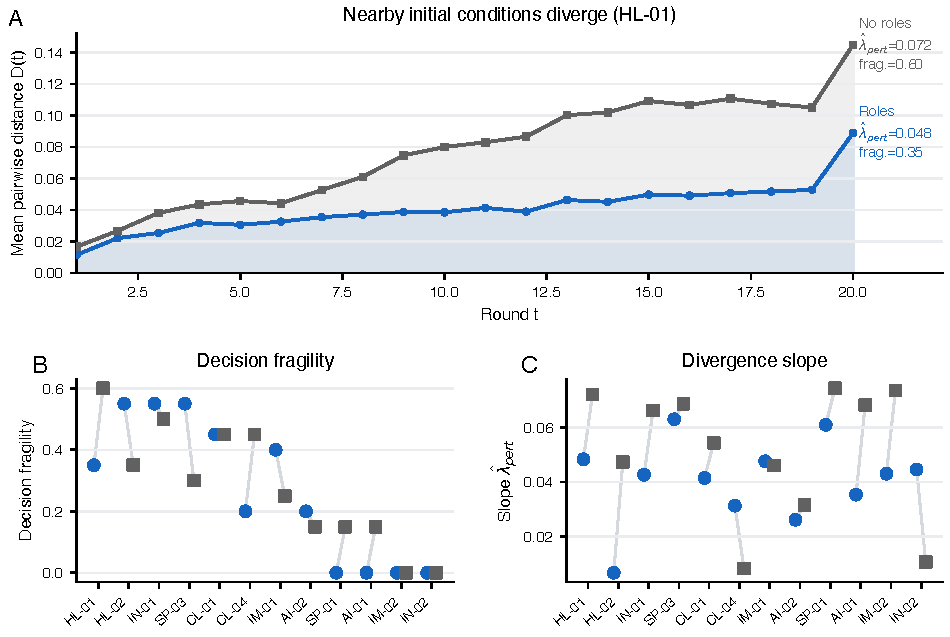
\includegraphics[width=\textwidth]{fig5_deterministic_hosted.pdf}
  \caption{\textbf{Small wording changes can redirect deterministic committees.}
  Hosted runs were executed in a fixed deterministic environment, and exact
  reruns of the same full 20-round committee pipeline were artifact-identical.
  (A) Mean pairwise trajectory distance $D(t)$ in HL-01 under
  meaning-conservative perturbations to the scenario text, shown separately for
  \Roles\ and \NoRoles. (B) Cross-scenario decision fragility under
  deterministic perturbations, defined as one minus the plurality share across
  20 variants. (C) Cross-scenario perturbation-divergence slope
  $\hat{\lambda}_{\mathrm{pert}}$. The variation therefore reflects controlled
  changes to initial conditions rather than stochastic reruns.}
  \label{fig:deterministic}
\end{figure}

\subsection*{Deployed committees vary, and design choices matter}

The deployed API experiments provide a practical counterpart to the hosted
benchmark. Prompts and settings were fixed and each condition was rerun up to
20 times at temperature 0. This regime does not isolate sensitivity to a small
input change as cleanly as the deterministic benchmark, because deployment-side
variation remains possible. It does, however, represent the setting in which
institutions are likely to use committee systems.

In HL-01, a uniform \NoRoles\ committee had a positive but comparatively low
divergence slope ($\lam=0.0221$). Adding role mandates to the same model
increased divergence ($\lam=0.0541$), and a mixed-model \NoRoles\ committee
was higher still ($\lam=0.0947$; Fig.~\ref{fig:architecture}A). The full
2$\times$2 matrix also shows that these factors do not follow a simple additive
rule: the mixed+roles condition was less unstable than mixed+no-role
($\lam=0.0519$ versus $0.0947$; Fig.~\ref{fig:architecture}B). The displayed
difference-in-differences estimate is local to HL-01 and is not evidence of a
scenario-general interaction. Across the broader scenario set, uniform
\NoRoles\ was usually the lowest-divergence configuration, but it often
remained in a positive-$\lam$ regime. Thus, temperature 0 should not be treated
as a guarantee of reproducible collective behavior (Supplementary Fig.~S8).

\begin{figure}[p]
  \centering
  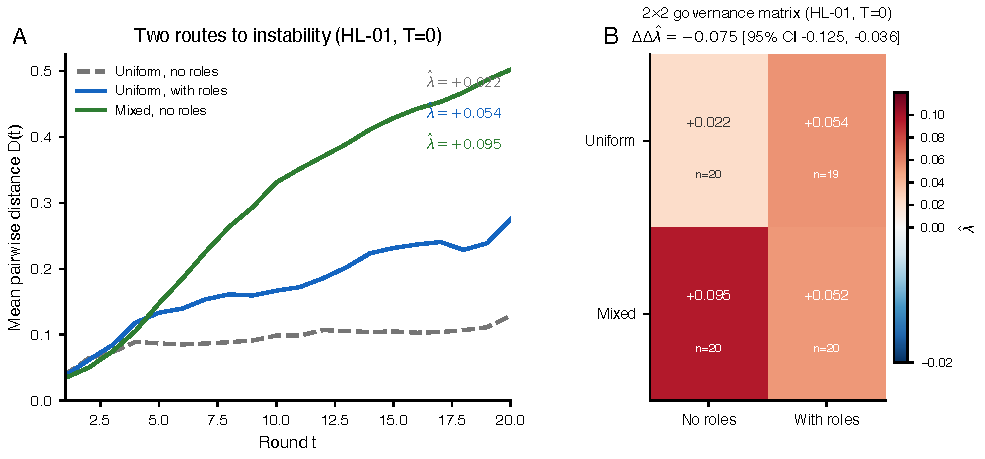
\includegraphics[width=\textwidth]{fig1_twopaths.pdf}
  \caption{\textbf{Committee design changes deployed instability (HL-01,
  $T=0$).} (A) Mean pairwise trajectory distance $D(t)$ for uniform \NoRoles,
  uniform \Roles, and mixed \NoRoles\ committees. Adding roles in a uniform
  committee and using mixed models without roles both increase divergence.
  (B) The 2$\times$2 matrix crosses role structure and model composition. The
  displayed difference-in-differences estimate and its 95\% replicate-bootstrap
  confidence interval define the HL-01 non-additivity check. Realized sample
  sizes are shown in cell; uniform+roles has $n=19$ and all other cells have
  $n=20$.}
  \label{fig:architecture}
\end{figure}

Role structure is one architectural channel, but not the only one. In
role-structured deployed committees, removing the Chair mandate produced the
largest reduction in HL-01 divergence among single-role ablations
(Fig.~\ref{fig:chair}A). Across five scenarios, the Chair effect was positive
in four, with the strongest and best-resolved effects in IM-01 and HL-01
(Fig.~\ref{fig:chair}B). This pattern does not make the Chair a universal source
of instability. It suggests that a synthesis-focused role can be an important
amplifier in this deployed, role-structured setting.

\begin{figure}[p]
  \centering
  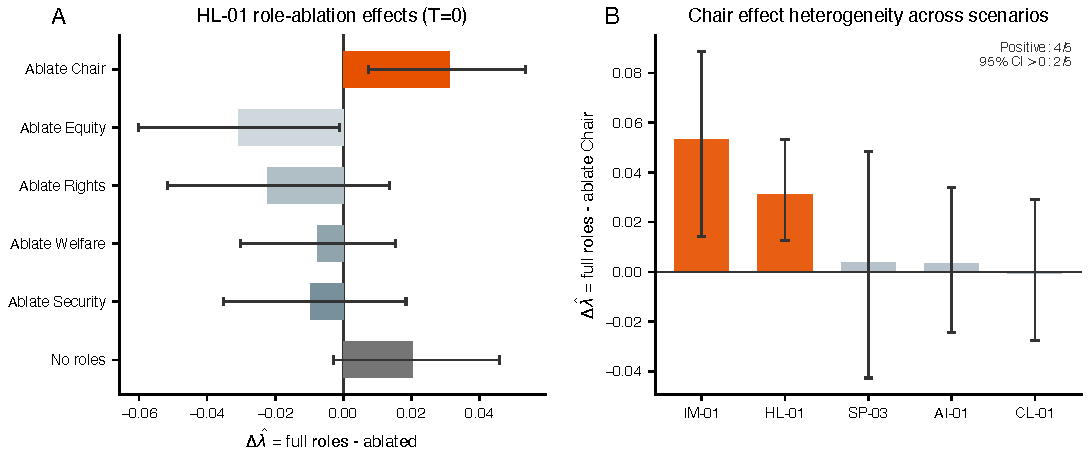
\includegraphics[width=\textwidth]{fig2_chair_mechanism_crossscenario.pdf}
  \caption{\textbf{The Chair role can amplify instability in role-structured
  deployed committees.} (A) HL-01 role-ablation effects on
  $\Delta\lam=\lam_{\mathrm{full\ roles}}-\lam_{\mathrm{ablated}}$.
  Chair ablation yields the largest reduction among role mandates, with a
  no-role reference shown for context. (B) Scenario-level Chair effects across
  IM-01, HL-01, SP-03, AI-01, and CL-01. Point estimates are positive in four
  of five scenarios, with strongest evidence in IM-01 and HL-01.}
  \label{fig:chair}
\end{figure}

\subsection*{Shorter memory is associated with less separation}

We next tested whether limiting access to earlier arguments changes the pattern.
Reducing argument-memory depth from $k=15$ to $k=3$ lowered $\lam$ in all four
tested scenarios (AI-01, CL-01, HL-01, and SP-03). A stricter memory-collapse
variant ($k=1$) also lowered $\lam$ relative to baseline \Roles\ in IM-01 and
CL-01 (Fig.~\ref{fig:memory}). These tests do not eliminate divergence and do
not isolate memory alone, because a shorter window also gives each agent less
information. They nevertheless provide descriptive evidence that stability is
partly a matter of deliberation protocol.

\begin{figure}[p]
  \centering
  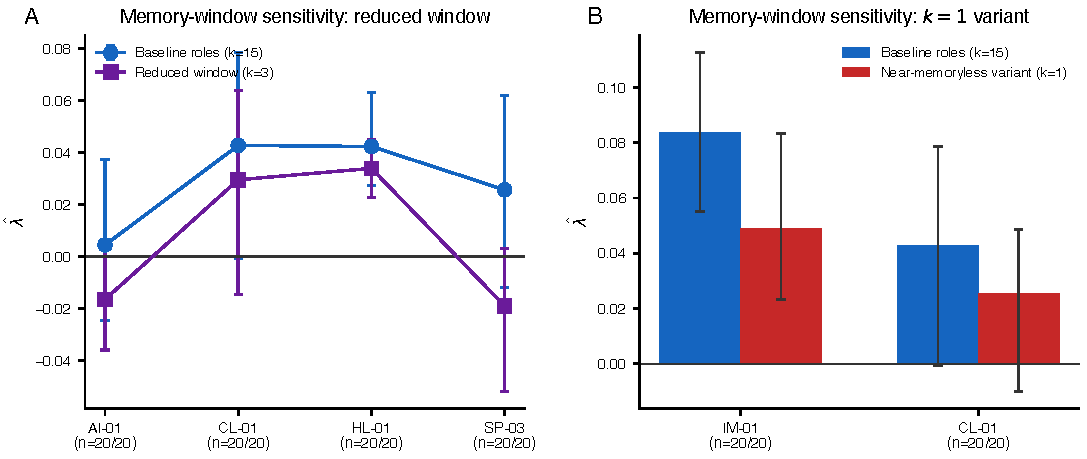
\includegraphics[width=\textwidth]{fig3_intervention_falsification.pdf}
  \caption{\textbf{Remembering less of the discussion is associated with less
  separation.} (A) Reducing the memory window from $k=15$ to $k=3$ lowers the
  point estimate of $\lam$ in all four displayed scenarios. (B) A $k=1$ variant
  likewise has lower point estimates in IM-01 and CL-01 than the $k=15$
  baseline. Whiskers show 95\% replicate-bootstrap confidence intervals and
  realized sample sizes are annotated in the panels. These descriptive
  interventions also change the information available to agents.}
  \label{fig:memory}
\end{figure}

\subsection*{Implications for auditing collective AI}

Multi-LLM committees are intended to make AI judgment more dependable: a group
may correct the errors or blind spots of a single model. Our results show a
limit to that intuition. Once agents repeatedly react to one another, the
discussion becomes a feedback process. Small changes can grow into different
lines of reasoning and sometimes different recommendations.

The deterministic benchmark makes the source of that problem clearer. Exact
reruns of the full pipeline were artifact-identical, removing residual execution
variation as an explanation. Yet wording changes that preserved the facts,
options, and endpoint still led committees apart over time and often changed the
recommendation. Repeatability, in other words, is not the same as robustness.

This matters for auditing and institutional use. A single transcript can be
coherent and persuasive while failing to represent what the same system would
recommend after an innocuous rephrasing. Auditing should therefore ask more than
whether one run is well reasoned. It should test whether the recommendation
survives nearby inputs that should not change the substance of the case. This
focus on measured and documented risk aligns with AI risk-management guidance
\cite{nist2023airmf}.

Our claims are empirical and deliberately bounded. The slope $\lam$ is an
operational index of growing separation, not a formal proof of deterministic
chaos \cite{eckmann1985ergodic,ott2002chaos}. We do not claim that every
multi-LLM committee is unstable for every task, model, or protocol. We show
instead that in this family of deliberative AI systems, instability can be
induced experimentally, modified by protocol choices, and survive deterministic
execution. The next step is to connect stability to consequences such as
accuracy, calibration, welfare, and decision harm, and to develop protocols that
limit unwanted amplification without eliminating useful disagreement.

\subsection*{Materials and methods}

\textbf{Protocol.} We used a windowed-summary deliberation protocol for
five-agent committees run over 20 rounds. At each round, every agent received
the scenario packet, a committee state table, and a transcript window of prior
arguments (default $k=15$), then returned free-form argument text and a
structured state line. A deterministic parser extracted preference vectors from
that state line, and one automatic repair pass was allowed after malformed
output.

\textbf{Scenarios.} The benchmark contains 12 structured policy scenarios
spanning immigration, health, income, climate, speech, and AI governance (two
scenarios per domain). Each scenario presents three discrete policy options and
a fixed decision endpoint.

\textbf{Models and conditions.} The deterministic hosted benchmark used
Qwen/Qwen2.5-7B-Instruct. The deployed API benchmark used GPT-4.1-mini for
uniform committees. Mixed-model committees used Chair (GPT-4.1), Welfare
(Claude Sonnet 4.6), Rights (Gemini 2.5 Flash), Equity (Grok-3-mini), and
Security (GPT-4.1-mini). Core deployed conditions crossed \NoRoles/\Roles\ with
uniform/mixed model composition at $T=0$. Additional deployed runs covered role
ablation and memory-window variants ($k=3$, $k=1$).

\textbf{Deterministic hosted extension.} The hosted benchmark used a fixed
single-GPU environment (NVIDIA L4, bfloat16), greedy decoding, single-process
execution, pinned seeds, and deterministic CUDA/PyTorch settings. Exact reruns
of the same committee condition were artifact-identical at the full-pipeline
level. Only the scenario text was perturbed through 20 manually screened,
meaning-conservative variants; committee instructions, parser schema, voting
logic, and execution settings were fixed.

\textbf{Inference and uncertainty.} For each condition, we computed the
committee mean trajectory and $D(t)$. In the deterministic benchmark, $D(t)$ was
computed across nearby prompt perturbations; in the API benchmark, it was
computed across nominal reruns at fixed settings. We estimated $\lam$ from
log-linear fits of $D(t)$ over rounds 3--20, and denote the hosted perturbation
analogue by $\hat{\lambda}_{\mathrm{pert}}$. Where reported, 95\% confidence
intervals were obtained from 500 bootstrap resamples of complete committee
trajectories. For the HL-01 2$\times$2 comparison, each cell was resampled
independently. Realized sample size is reported at panel or cell level. Reporting
follows reproducibility-oriented practice for empirical ML benchmarks
\cite{pineau2021improving}.

\textbf{Implementation.} Experiments and analyses were implemented in Python
3.11 with NumPy, SciPy, and Matplotlib \cite{scipy2020,matplotlib2007}.

\clearpage
\bibliography{refs}
\bibliographystyle{sciencemag}

\section*{Acknowledgments}
\paragraph*{Funding:}
W.K. is financially supported by the FRQ-IVADO Research Chair Program and the
Fonds de Recherche du Québec -- Société et Culture (FRQSC) Research Team Support
Grants (Grant no. 380210).
\paragraph*{Author contributions:}
H.S. and W.K. conceptualized the study. H.S. developed the methodology. H.S. and
S.K. conducted the formal analysis and investigation. H.S. and W.K. prepared the
original draft. H.S. and S.K. reviewed and edited the manuscript. W.K.
supervised the study.
\paragraph*{Competing interests:}
The authors declare no competing interests.
\paragraph*{Data and materials availability:}
The run artifacts, input materials, and analysis code supporting the findings
are publicly available at
\url{https://github.com/shimaohajime/Collective-AI-divergence}.

\section*{Supplementary materials}
Materials and Methods S1 to S6\\
Supplementary Figures S1 to S8\\
Supplementary Tables S1 to S8

\end{document}
